\documentclass[a4paper, titlepage, oneside, 12pt]{article}%      autres choix : book  report

\usepackage[utf8]{inputenc}%           gestion des accents (source)
\usepackage[T1]{fontenc}%              gestion des accents (PDF)
\usepackage[francais]{babel}%          gestion du français
\usepackage{textcomp}%                 caractères additionnels
\usepackage{mathtools,  amssymb, amsthm}% packages de l'AMS + mathtools
\usepackage{lmodern}%                  police de caractère
\usepackage{geometry}%                 gestion des marges
\usepackage{graphicx}%                 gestion des images
\usepackage{xcolor}%                   gestion des couleurs
\usepackage{array}%                    gestion améliorée des tableaux
\usepackage{calc}%                     syntaxe naturelle pour les calculs
\usepackage{titlesec}%                 pour les sections
\usepackage{titletoc}%                 pour la table des matières
\usepackage{fancyhdr}%                 pour les en-têtes
\usepackage{titling}%                  pour le titre
\usepackage[framemethod=TikZ]{mdframed}% print frames
\usepackage{caption}%                  for captionof
\usepackage{listingsutf8}

\usepackage{enumitem}%                 pour les listes numérotées
\usepackage{microtype}%                améliorations typographiques
\usepackage{csvsimple}%                 convertir un fichier .csv en tableau


\usepackage{hyperref}%                 gestion des hyperliens

\usepackage{titling} %  				  gestion des subtitles 
\newcommand{\subtitle}[1]{%			  definition d'une nouvelle commande sous-titre
  \posttitle{%
    \par\end{center}
    \begin{center}\large#1\end{center}
    \vskip0.5em}%
}                
\lstset{language=c++}
\definecolor{codegreen}{rgb}{0,0.6,0}
\definecolor{codegray}{rgb}{0.5,0.5,0.5}
\definecolor{codepurple}{rgb}{0.58,0,0.82}
\definecolor{backcolour}{rgb}{0.95,0.95,0.92}
 
\lstdefinestyle{mystyle}{
    backgroundcolor=\color{backcolour},   
    commentstyle=\color{codegreen},
    keywordstyle=\color{magenta},
    numberstyle=\tiny\color{codegray},
    stringstyle=\color{codepurple},
    basicstyle=\footnotesize,
    breakatwhitespace=false,         
    breaklines=true,                 
    captionpos=b,                    
    keepspaces=true,                 
    numbers=left,                    
    numbersep=5pt,
    otherkeywords={uint16_t},                  
    showspaces=false,                
    showstringspaces=false,
    inputencoding=latin1,
    showtabs=false,                  
    tabsize=2
}
\lstset{style=mystyle}

\hypersetup{%
    pdfborder = {0 0 0}
}

                                    
\title{Projet PERI :\\ Dispositif météorologique}
\subtitle{Rapport de projet}

\author{ Paul MABILLOT \& Adrien FERREIRA \& Pierre MAHÉ}
\date{\today}


\begin{document} 

\begin{figure}[h]
\maketitle 
\end{figure}

\begin{figure}[b]
	
\includegraphics[width=100px] {upmc_logo.jpg}
\end{figure}

\newpage   
   
\tableofcontents

\newpage

\section{Description du projet}
\section{Montage}
\subsection{Arduino}

\paragraph{}
Faire le montage suivant votre carte Arduino. \\ 
Pour les cartes Nano et One les branchements sont similaire. À noter que nous n'utilisons pas de led externe mais celle intégrée au circuit.
\newline
\\
	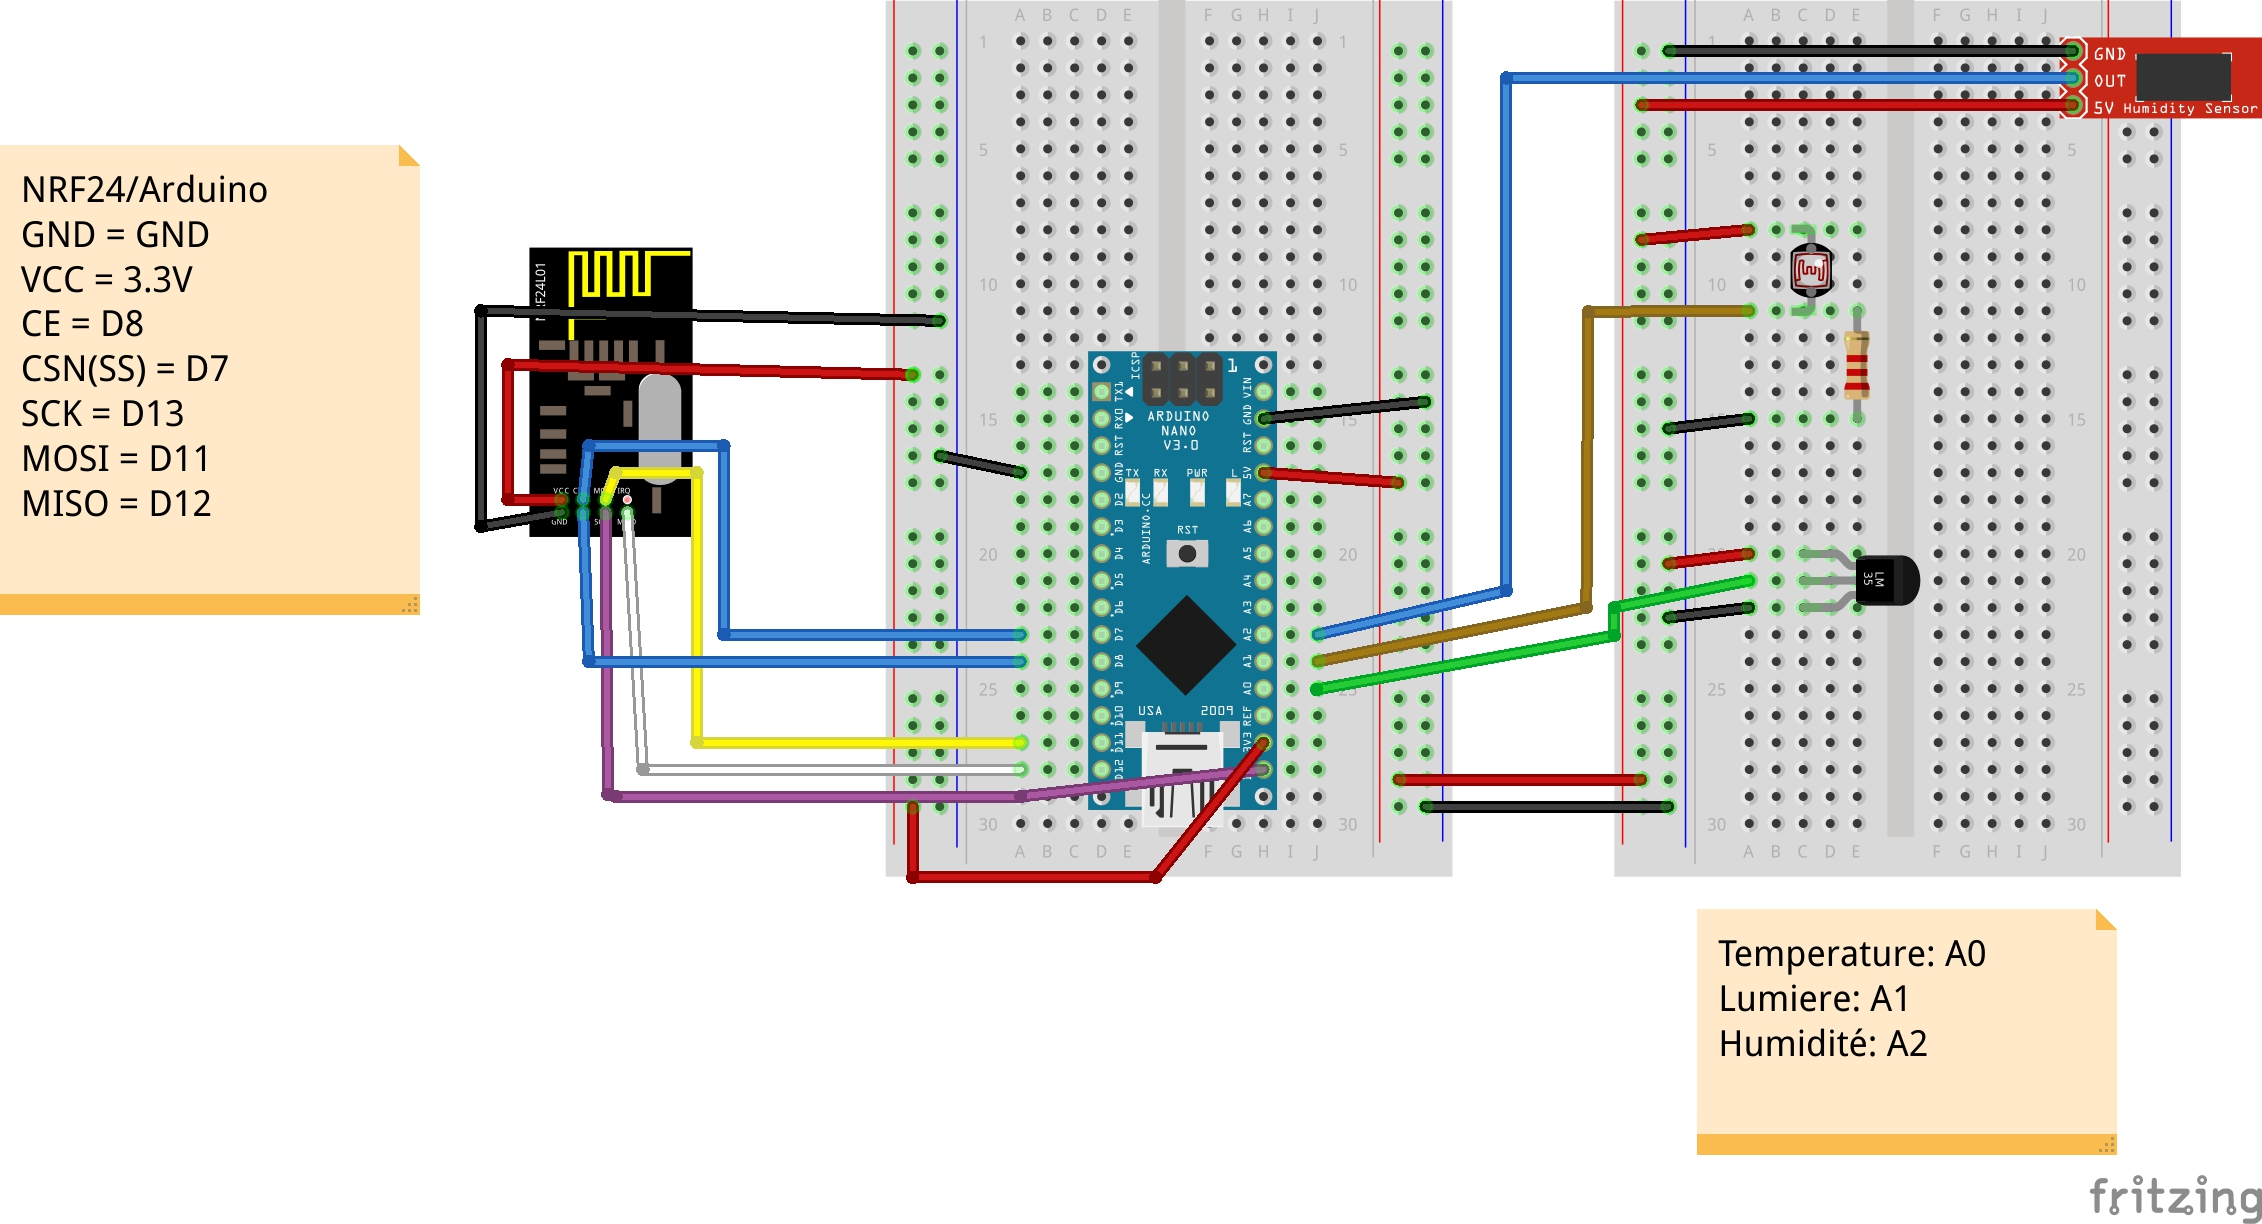
\includegraphics[width=400px] {montage-arduino-nrF24.jpg}

\paragraph{}
Pour l'arduino Mega le montage est un peu différent.
Branchez le pin CSN(SS) au pin D53, le SCK au pin D52, le MOSI au pin D51 et le MISO au pin D50.
\newline
\\
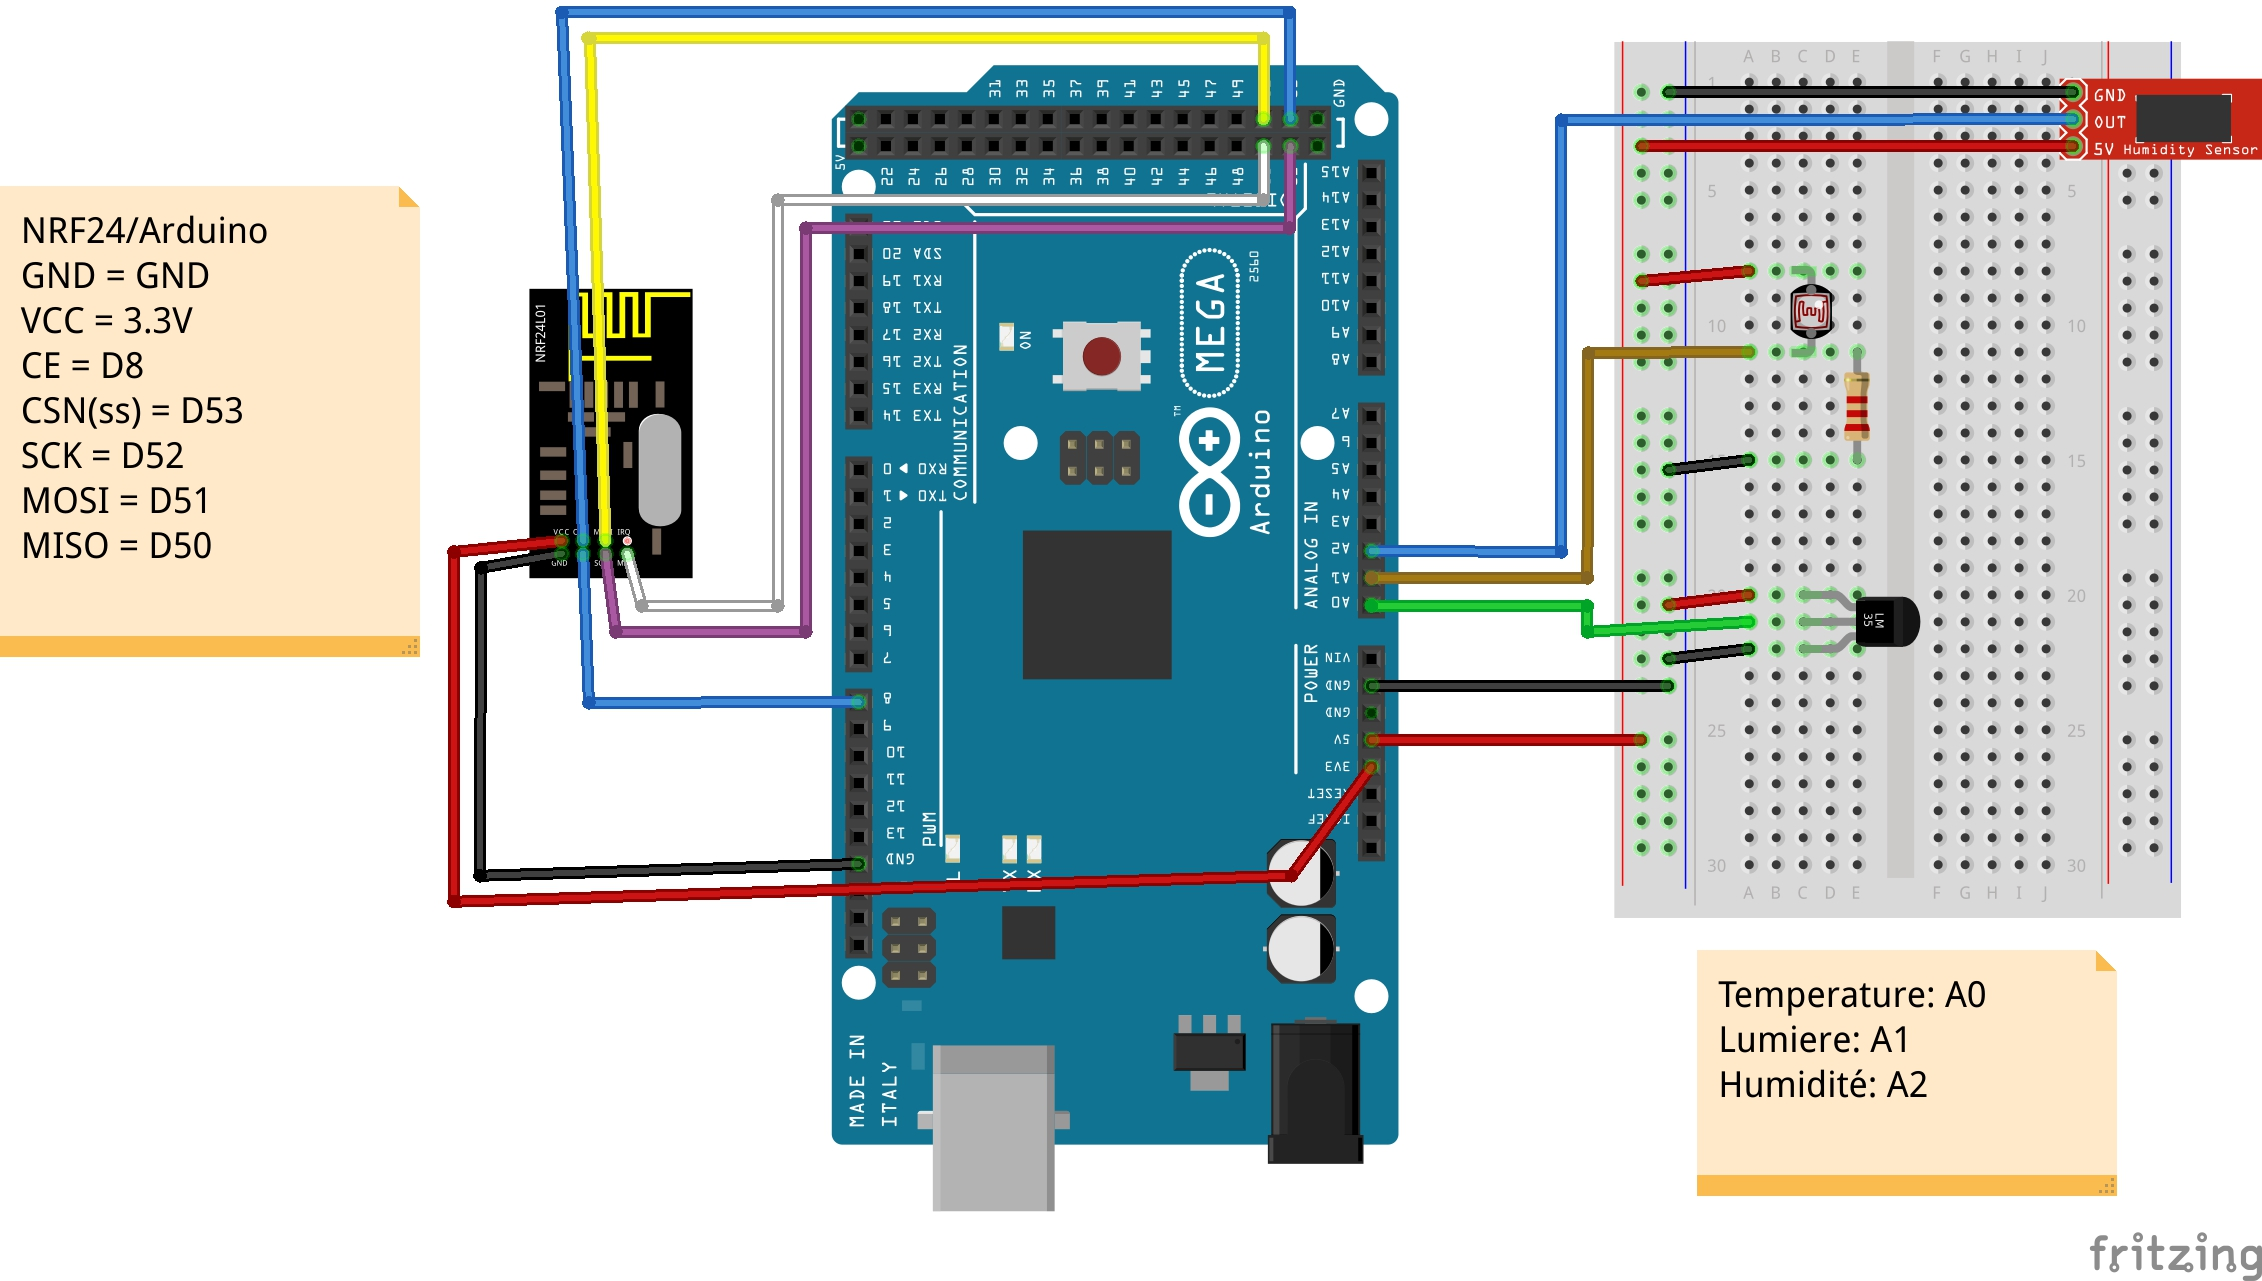
\includegraphics[width=400px] {montage-arduino-mega-nrF24.jpg}

\subsection{Raspberry Pi}
\paragraph{}
Faire le montage suivant sur votre carte Raspberry Pi.\\ Dans cet exemple, nous avons utilisé une Raspberry Pi modèle B mais pour les modèles B+ et 2 la retro-compatibilité est assurée, il suffit de procéder au même branchement que le schéma.
\newline
\\
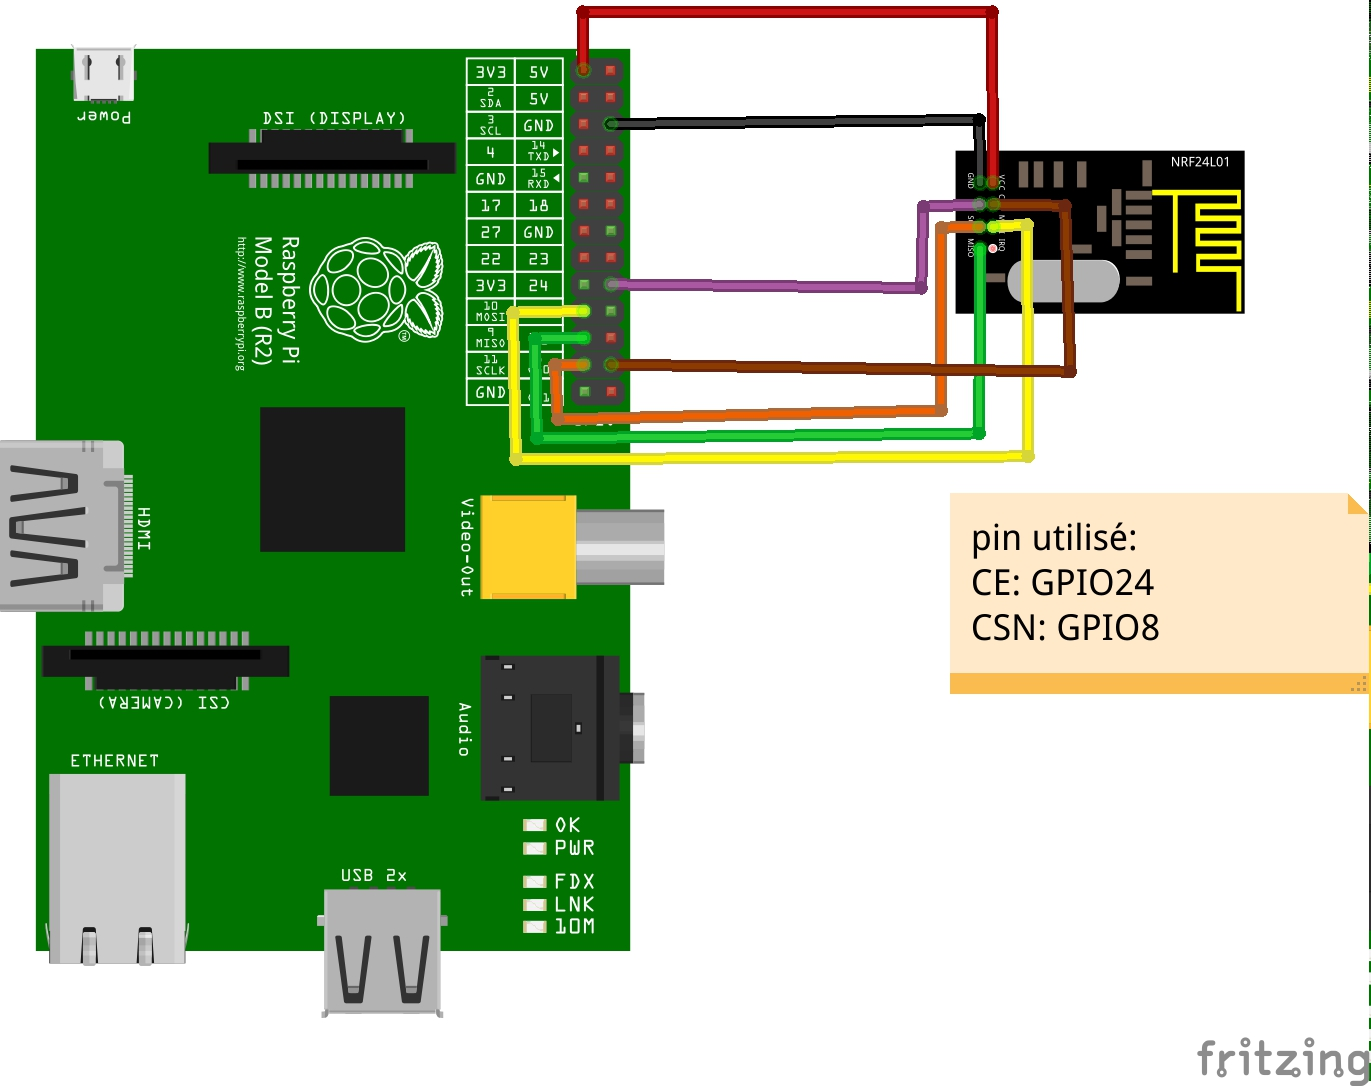
\includegraphics[width=400px] {montage-raspberry-nrF24.jpg}

\paragraph{}
\textbf{Attention: Le module nRF24 est fragile, il n'accepte qu'une alimentation 3.3V, ne surtout pas le brancher sur le pin 5V au risque de l'endommager.}

\section{Codage}
\subsection{Structure de données}
Cette structure est commune aux deux cartes, elle permet de structurer les données envoyées.
\begin{lstlisting}
typedef struct t_payload{
	uint16_t cmd;
	uint16_t timeStamp;
	uint16_t valLight;
	uint16_t valTemperature;
	uint16_t valHumidity;
} payload;
\end{lstlisting}
%TODO changer t_payload
Pour garantir l’interopérabilité, il est impératif de définir explicitement la taille des types manipulés.
\textbf{Attention: certains compilateurs rajoutent des octets de bourrage pour aligner la taille de la structure en mémoire. Veillez donc à accorder les options des deux compilateurs (Arduino et Raspberry).}
L'option \texttt{packed} peut être utilisée comme directive pour le compilateur.
  
L'endianess de l'Arduino et la Raspberry étant identique il n'a pas été nécessaire d'opérer à des conversions, attention cependant au portage sur d'autres systèmes.
\texttt{cmd} utile pour définir le type de traitement à réaliser (cf: Protocole).
Les autres champs sont présent pour stocker les données à proprement parler.
\subsection{Arduino}
\paragraph{}
Pour envoyer les données a intervalle reguliere, vous devez installer la bibliothèque \href{http://playground.arduino.cc/Code/SimpleTimer?ref=driverlayer.com/web}{\textit{SimpleTimer}} (téléchargeable sur le site officiel Arduino).\\
Il faut tout d'abord armer un timer avec un temps (en milliseconde) et un pointeur de fonction (sans paramètre) dans le \texttt{setup}. Dans le \texttt{loop}, appelez la fonction \texttt{run}.\\
\begin{lstlisting}
SimpleTimer timer;
timer.setInterval(DELAY, fctnCallback);
timer.run()
\end{lstlisting}


\paragraph{}
Pour communiquer avec la module nRF24L01+, vous devez installer une seconde bibliothèque.
\href{https://github.com/stanleyseow/RF24}{\textit{lien du dépôt}}. Seul les fichiers \texttt{RF24.cpp} et \texttt{RF24.h} sont à copier dans le dossier \texttt{libraries} de l'IDE sketch.
\\ \\
\subsubsection{Initialisation}
La sequence d'instruction à utiliser pour initialiser le module nRF24 est:\\

\begin{lstlisting}
radio.begin();
radio.setPALevel(RF24_PA_MAX);	// la force d'emission du signal
radio.setDataRate(RF24_1MBPS);	// le debit de donnees

// identifiant arbitraire du canal de emission 
radio.openWritingPipe(0x0000000001LL);
// identifiant du canal de reception pour le pipe 1
radio.openReadingPipe(1, 0x0000000002LL);
\end{lstlisting}
\paragraph{}
\textbf{Attention: Il n'est possible d’écouter que sur 6 canaux simultanément.\\}
Attention à correctement synchroniser les canaux utilisés par les nœuds. Si deux modules écrivent sur le même canal, des collisions vont apparaître.

\subsubsection{Lecture}
Avant de pouvoir envoyer des données grâce au module nRF24, il faut l'activer en lecture grâce à l'instruction : \texttt{startListening()}.
Pour savoir si une donnée est en attente dans le buffer de réception, il faut utiliser l'instruction \texttt{avaiable()} non-bloquante.
Pour récupérer la valeur, il faut utiliser \texttt{read}.

\subsubsection{Écriture}
Il n'est pas possible d'écouter et d'émettre simultanément. De ce fait, avant une écriture, il faut prendre soin d'appeler \texttt{stopListening()} pour arrêter l'écoute. Ensuite, utilisez \texttt{write()} pour envoyer les données.
Ne pas oublier de réactiver l'écoute ensuite.

\subsection{Raspberry Pi}
Pour communiquer avec la module nRF24L01+ depuis la Raspberry, utilisez les fonctions présentes dans les fichiers \texttt{RF24.cpp}, \texttt{RF24.h}, \texttt{bcm2835.c} et \texttt{bcm2835.h}.

\subsubsection{Initialisation}
\paragraph{}
La phase d'initialisation est similaire à celle de l'Arduino. 

\begin{lstlisting}
/* les deux premiers arguments sont les pins GPIO a utiliser pour CE et CS (definie BCM2835.h) la cadence du pin SPI.*/
RF24 radio(BCM2835_SPI_CS_GPIO24, 800000, BCM2835_SPI_SPEED_8MHZ);
radio.begin();
radio.setPALevel(RF24_PA_MAX);		// la force d'emission du signal
radio.setDataRate(RF24_1MBPS);		// le debit de donnees

// identifiant du canal de reception pour le pipe 1
radio.openReadingPipe(1,0x0000000001LL);		
// identifiant arbitraire du canal de emission 
radio.openWritePipe(0x0000000002LL);

radio.startListening();
\end{lstlisting}

\subsubsection{Lecture, écriture}
\paragraph{}
La manière de procéder et les fonctions à appeler sont les mêmes que pour l'Arduino.

\section{Protocole de niveau applicatif}
Pour pouvoir synchroniser les horloges des deux cartes, nous avons créé un protocole simple.
Au démarrage l'Arduino envoi un message avec \texttt{cmd = INIT } et se met en attente de la réponse de la Raspberry. Quand elle reçoit ce paquet la Rasperry répond avec son estampille temporelle dans \texttt{timestamp} et \texttt{cmd = INIT}. L'Arduino sauvegarde cette valeur et l'utilisera pour dater ses envois (en l'incrémentant).
De ce fait, si la carte Arduino venait à s'éteindre, elle cherchera à se re-synchroniser au démarrage.
Suite à cela, l'Arduino pourra envoyer ses valeurs de capteur avec \texttt{cmd = DATA} et les autres champs remplis en conséquence.


\section{Serveur}
\subsection{Installation}
\paragraph{}
Dans cette partie, nous allons nous pencher sur code. Par un soucis de lisibilité nous n'allons pas commenter toute les fonctions, nous indiquerons autant que faire se peu les noms des fichiers et des fonctions, à vous de regarder dans les fichiers du projet le code exacte.
\paragraph{}
-Installation Apache2 et PHP
\begin{lstlisting}
sudo apt-get install apache2 php5 libapache2-mod-php5
\end{lstlisting}
\paragraph{}
-Installation Mysql (inutile dans notre cas)
\begin{lstlisting}
sudo apt-get install mysql-server php5-mysql
\end{lstlisting}
-Installation Mysql (inutile dans notre cas)
\begin{lstlisting}
sudo apt-get install mysql-server php5-mysql
\end{lstlisting}
-Répertoire du serveur
\begin{lstlisting}
/var/www/
\end{lstlisting}

Commandes Serveur:
\begin{lstlisting}
$service apache2 stop : arreter serveur
$service apache2 start : demarrer serveur
$service apache2 restart : redemarrage serveur
\end{lstlisting}

\subsection{Mise en place}
\subsubsection{Création de l'index.php}
\paragraph{}
Dans un premier temps nous allons créer la page d’accueil de notre station météo.
On souhaite y afficher les informations en temps réel ainsi qu'un graphique regroupant les informations des derniers jours.\\ \\ 
Dans la section \textit{"station"} nous afficherons les données\\
Dans la section \textit{"recap"} nous afficherons le graphique\\


\begin{lstlisting}
<!DOCTYPE html>
		<html>
			<head>
			<meta name="description" content="Bienvenue sur le site de meteorologique SAR" />
			<meta charset="utf-8" />
			<link rel="stylesheet" href="css/style.css" />
			<title>Site meteorologique</title>
			</head>

			<body>
			<section id="meteo">
				<h1>Station Meteo</h1>
			
				<section id="station">
				</section>
				
				<section id="recap">				
				</section>
			</section>
			</body>
		</html>
\end{lstlisting}

Votre raspbery ne sera pas forcement connecté à internet, il est donc important d'importer les librairies pour assurer le bon fonctionnement de votre station météo même hors ligne.\\
C'est pour cela que nous avons choisi la bibliothèque jquery et jqPlot.\\ Le code suivant est a ajouter dans le \textit{<head>}.
\paragraph{}
La librairie jquery :
\begin{lstlisting}
<script src="js/jquery-1.11.2.min.js"></script>	
\end{lstlisting}
La libraire de gestion de graphique jqPlot:
\begin{lstlisting}
	<script type="text/javascript" src="js/jqPlot/jquery.jqplot.min.js"></script>	
    	<script type="text/javascript" src="js/jqPlot/plugins/jqplot.canvasTextRenderer.min.js"></script>
	<script type="text/javascript" src="js/jqPlot/plugins/jqplot.canvasAxisLabelRenderer.min.js"></script>	
\end{lstlisting}

\subsubsection{Récupération de la valeur}
\paragraph{}
Les données envoyés par votre arduino sur votre raspberry (voir plus haut) sont sauvegardés dans le fichier xml/fichier.xml de votre serveur apache. Nous allons écrire une fonction PHP permettant de récupérer la dernière valeur ajoutée dans ce fichier.
\begin{lstlisting}
function getLastValue($path){
		$fp = fopen($path, "r");
		
		if (flock($fp, LOCK_SH)) {
			$xml = simplexml_load_file($path);
			flock($fp, LOCK_UN);
			$taille = sizeof($xml);
			$last = $xml->timestamp[$taille-1];	
		}
		return $last['valeur'].' '.$last->temperature.' '.$last->humidite.' '.$last->luminosite;
	}	
\end{lstlisting}
\paragraph{}
La fonction getLastValue, qui prend en paramètre le chemin vers votre fichier XML, s'occupe d'ouvrir ce fichier en lecture seul.\\
On verrou est alors placé pour éviter une écriture durant la lecture.\\
La fonction \texttt{simplexml\_load\_file} s'occupe de parser un fichier XML et retourne un objet facilement navigable.\\
Une fois l'objet obtenu on relâche le verrou. \\
On s'occupe de récupérer le nombre total d’élément dans le fichier XML afin de récupérer le dernier timestamp que l'on stock.\\
La fonction retourne alors le timestamp, la température, l'humidité et la luminosité du dernier envoi.\\

\subsubsection{Rafraîchissement automatique}
\paragraph{}
Afin de rendre notre page dynamique nous souhaitons que les derniers valeurs envoyés par nos sondes soient directement affichés. Pour cela nous allons utilisé notre fonction PHP écrite précédemment.\\
Malheureusement comme le PHP est géré coté serveur il est impossible de réaliser cela sans l'aide de javascript.\\
Pour cela, il faut utiliser le fichier \texttt{getLast.php} qui va lui même appeler le fichier \texttt{loadData.js}, Qui va appeler toute les 1000ms une fonction qui va retourner les nouvelles valeurs du timestamp, de la temperatuyre, de l'humidité et de la luminosité.\\
Il ne bous reste plus qu'à traiter ces données.\\
Pour la luminosité on avons decider de faire l'approximation suivant: si il y a beaucoup de lumière alors on peut considérer qu'il fait beau si au contraire il y a peu de lumière alors nous pouvons dire que le temps est couvert. De plus nous avons ajouter un balance jour/nuit (cf. fonction \texttt{traitementLumino}).
Le traitement permet de charger des différentes images dans le html, selon le temps qu'il fait.

\subsubsection{La partie Graphique}
\paragraph{}
 Nous afficherons les données des 3 derniers jours sur notre graphique lors du chargement de la page. Pour cela nous savons que chaque information est reçu toute les 1s, il faut donc traiter 86400 événements par jour, soit dans notre cas 259200 événements (60*60*24*3) (cf. \texttt{loadGraphe.php}).\\
Nous ne souhaitons pas réafficher le graphique après chaque réception de donnée, cela serai trop lourd pour notre serveur.\\ Contrairement aux données, nous recalculons le graphique qu'au moment du rafraîchissement de la page par le navigateur web. \\
Nous avons utiliser un fonction javascript pour afficher le graphique.
\begin{lstlisting}
function getAllValues()
\end{lstlisting}
Comme précédemment la fonction ouvre le fichier XML, positionne le verrou, mais ici elle va sauvegarder uniquement les données des 259200 événements disponibles et retourner un tableau.\\
Afin de fournir ces données à la bibliothèque \textit{jqPLot}, voir le fichier \texttt{loadGraph.php}.
\begin{lstlisting}
<?php 
	include("gestionFile.php"); 
	/* Recuperer les timestamp dans le fichier XML */
	$res = getAllValues("xml/fichier.xml");
	$tabjs = php2js($res);
?>
\end{lstlisting}
Le code PHP récupères les données et les mets en forme pour le javascript à l'aide de la fonction \textit{php2js}.\\
\subsubsection{Bonus}
\paragraph{}
Il est possible de faire de la mise ne page en ajoutant des feuilles de style.
\end{document}




